\documentclass[12pt, conference, compsocconf]{IEEEtran}

\usepackage{amsmath, amsfonts}
\usepackage{graphicx}
\usepackage{url}
\usepackage{tikz}
\usepackage{color, soul}

%%% Package and definitions for displaying pseudocode
\usepackage{algorithm}
\usepackage[noend]{algpseudocode}
%\newcommand*\Let[2]{\State #1 $\gets$ #2}
%\algrenewcommand\alglinenumber[1]{
%    {\sf\footnotesize\addfontfeatures{Colour=888888,Numbers=Monospaced}#1}}
%\algrenewcommand\algorithmicrequire{\textbf{Precondition:}}
%\algrenewcommand\algorithmicensure{\textbf{Postcondition:}}


\begin{document}
\title{CISC-481/681 Project 2: A* Search with Heuristics}

\author{\IEEEauthorblockN{Dylan Chapp, Michael Wyatt}
\IEEEauthorblockA{Department of Computer and Information Sciences \\ University
of Delaware - Newark, DE 19716 \\ Email: \{dchapp\}, \{mwyatt\}@udel.edu}}

\maketitle

\section{Introduction}
In this work we implement the A* search algorithm to solve the problem of
directing a predator (e.g., a cat) through a maze of obstacles to multiple prey
objectives (e.g., mice).  We introduce heuristics specifically tailored to this
multi-objective pathfinding problem and provide an empirical evaluation of
their performance.

\section{Related Work}
The problem presented in this report is analagous to the Traveling Sales Person
(TSP) problem.  In TSP, we must find the shortest route between the
sales person's home, through several cities and back.  It is trivial to reduce
the cat and mouse problem to TSP; Therefore, the problem we are solving in this
report is an NP-Complete problem, just like TSP.

The A* search algorithm has been used to solve problems like TSP, as well as
many other applications.  For example, A* is often used in video games for NPC
map traversal.  A* was developed as an extension to Dijkstra's algorithm and
can be used for any general graph or tree search problems.

\section{Problem Characterization}
We are presented with the problem of providing a cat with a shortest path that
allows it to navigate to and consume $m$ mice on an $n \times n$ board of
tiles.  However, some of these tiles are obstacles that the cat cannot
traverse, which makes computing shortest paths nontrivial.  We employ the A*
search algorithm to find, for a fixed starting tile and a fixed goal tile
containing a mouse, a shortest path for the cat.  In turn, we use heuristics
for executing repeated applications of single-objective A* search to find a
shortest path to all of the mice.

\section{The A* Algorithm}
A* is an informed search algorithm used for finding the shortest path from a
single node in a graph--the start--to some other node in the graph--the goal.
Specifically, A* constructs a tree whose root is the start node and one of
which's leaves is the goal node.

The A* algorithm bears resemblance to uninformed search algorithms such as
breadth-first search in terms of its general structure, but differs in that it
maintains a priority queue of nodes to expand upon rather than a FIFO/LIFO
queue.  The priority queue is ordered according to a heuristic that accounts
for both the known cost to reach a node from the starting node and the
estimated cost to reach the goal node from that node.

In fact, A* was developed as an improved upon Dijkstra's algorithm, a similiar
search algorithm that too maintains a priority queue of nodes, but orders them
only with respect to the known cost to reach them from the starting node.
Below,~\ref{alg-astar} we provide pseudocode for A*, highlighting how A* uses 
the the path cost, which is used in Dijkstra's algorithm, \emph{and} a heuristic 
function $h$ to prioritize nodes in the frontier. 

\begin{algorithm}
    \caption{A* Search}
    \label{alg-astar}
    \begin{algorithmic}[1]
        \Function{A*}{start, goal, $h$}
            \State $\text{explored} \gets \{\}$
            \State $\text{frontier} \gets \text{PriorityQueue()}$
            \State $\text{frontier.insert(start, 0)}$
            \State $\text{costToReach} \gets \text{HashMap()}$
            \State $\text{parent} \gets \text{HashMap()}$
            \State $\text{costToReach}[\text{start}] = 0$
            \State $\text{parent}[\text{start}] = Nil$
            \While{frontier not empty}
                \State $current \gets \text{frontier.pop()}$
                \If{current == goal}
                    \State{break}
                \Else
                        \For{$n \in current.neighbors()$}
                        \State $\text{cost} \gets \text{costToReach[current]} + 1$
                        \If {$n \notin \text{costToReach}$ or \\ \hspace{1in}cost $<$ costToReach[n]}
                                \State costToReach[n] = cost
                                \State \hl{$p = \text{cost} + h(\text{goal}, n)$}
                                \State frontier.insert($n$, $p$)
                                \State parent[n] = current
                            \EndIf
                        \EndFor
                \EndIf
            \EndWhile
        \State \Return{parent, costToReach}
        \EndFunction
    \end{algorithmic}
\end{algorithm}

\subsection{Single Objective A* Heuristics}
We developed two valid heuristics for A*.  Both are valid because they
consistently underestimate the real cost of reaching a goal node from a given
start position.  Each heuristic is able to handle cases when there are multiple
goals.  The heuristics will help guide A* to the nearest goal on the board by
returning the minimum estimated distance between a start position and any goal.
The first heuristic calculates the manhattan distance between a position and
goals.  The manhattan distance is the number of moves--up, down, left, or
right-- that the cat must make to reach a goal.  If there are no obstacles
present, it is also an exact solution for the cost to a given goal.  The
psuedocode for this heuristic can be seen in algorithm~\ref{manhattan}.

\begin{algorithm}
    \caption{Manhattan distance heuristic}
    \label{manhattan}
    \begin{algorithmic}[1]
        \Procedure{Manhattan}{start, goals}
        \State $minDist\gets \infty$
        \State $(x_1, y_1)\gets start$
        \For{$goal \in goals$}
        \State $(x_2, y_2)\gets goal$
        \State $dist\gets \lvert x_2-x_1\rvert + \lvert y_2-y_1\rvert$
        \State $minDist\gets min(dist, minDist)$
        \EndFor
        \Return $minDist$
        \EndProcedure
    \end{algorithmic}
\end{algorithm}

The second heuristic calculates the euclidean distance between a start position
and goals.  The euclidean distance is the straight-line distance between any
two points.  This heuristic will always underestimate the distance to a
goal for this problem.  Pseudocode for the euclidean distance can be seen in
algorithm~\ref{euclidean}.

\begin{algorithm}
    \caption{Euclidean distance heuristic}
    \label{euclidean}
    \begin{algorithmic}[1]
        \Procedure{Euclidean}{start, goals}
        \State $minDist\gets \infty$
        \State $(x_1, y_1)\gets start$
        \For{$goal \in goals$}
        \State $(x_2, y_2)\gets goal$
        \State $dist\gets \sqrt{(x_2-x_1)^2+(y_2-y_1)^2}$
        \State $minDist\gets min(dist, minDist)$
        \EndFor
        \Return $minDist$
        \EndProcedure
    \end{algorithmic}
\end{algorithm}

\subsection{Multi Objective A* Heuristics}
The A* algorithm and associated heuristics described thus far are able to
handle multiple objectives, but will only find the path between a starting
point and the nearest goal. If we want to contruct the path from a starting
point to all goals, we need a heuristic for utilizing our single objective A*
implementation.  To achieve a path from the starting point through all goals,
we implemented two different multi-objective heuristics.

The first heuristic is a na\"{\i}ve implementation of multi-objective A*.  A
path to all goals is built by finding the subpath between a start point and its
Nearest Neighbor (NN), which is also a goal.  This is accomlished through
iterative calls to the A* algorithm while changing the start position to the
previously found goal.  Psuedocode for this multi-objective heuristic can be
found in algorithm~\ref{nna}.

\begin{algorithm}
    \caption{NN multi-objective A*}
    \label{nna}
    \begin{algorithmic}[1]
        \Procedure{NearestGoalAStar}{start, goals}
        \State $path\gets []$
        \While{$goals$ not empty}
        \State $goal, subPath\gets A*(start, goals)$
        \State append $subPath$ to $path$
        \State $start\gets goal$
        \State remove $goal$ from $goals$
        \EndWhile
        \Return $path$
        \EndProcedure
    \end{algorithmic}
\end{algorithm}

The second heuristic works by exhaustively searching all possible paths and
returning the path which touches each goal and has the lowest cost.  This path
can thought of as a Minimum Spanning Path (MSP) for the start and goals.  The
algorithm first builds a library of all possible subpaths between any two
points in the set of start and goal positions.  Using this library, it then
builds all possible paths of an appropriate length ($len(goals)-1$).  The
algorithm then removes any path which does not visit all goals and the start
position (i.e., a complete path.)  A path cost for each of these paths is then
computed and the path with the minimum cost is returned.  Pseudocode for this
multi-objective heuristic can be found in algorithm~\ref{ca}.

For the pseudocode in algorithm~\ref{ca}, the function
$CompletePaths(subPaths)$ builds all possible paths of length $length(goals)-1$
and returns only the complete paths.  The fuction $GetPathCost(path, cost)$
calculates the cost of a path using the path and a list of costs for all
subpaths.

\begin{algorithm}
    \caption{MSP multi-objective A*}
    \label{ca}
    \begin{algorithmic}[1]
        \Procedure{CombinatorialAStar}{start, goals}
        \State $cost \gets []$
        \State $subPaths\gets$ combinatorial pairs of $\{start, goals\}$
        \For{$subPath \in subPaths$}
            \State $(start, goal) \gets subPath$
            \State $pathCost \gets A*(start, goal)$
            \State append $pathCost$ to $cost$
        \EndFor
        \State $paths\gets CompletePaths(subPaths)$
        \State $minCost \gets \infty$
        \State $minPath \gets NULL$
        \For{$path \in paths$}
            \State $pathCost \gets GetPathCost(path, cost)$
            \If{$pathCost < minCost$}
                \State $minPath\gets path$
                \State $minCost\gets cost$
            \EndIf
        \EndFor
        \Return $minPath$
        \EndProcedure
    \end{algorithmic}
\end{algorithm}

\section{Implementation}
We implemented our core single-objective A* search algorithm, all helper
functions for ingesting and reporting data, and all functions necessary to
adapt the single-objective algorithm to the multi-objective problem posed in
Python.  This choice was guided by the authors' familiarity with the language
and the knowledge that we would be able to rapidly iterate on and test our
design.  With the exception of a few uses of the NumPy numerical computation
module for convenience, the project is implemented without the use of 3rd-party
modules.

\subsection{Components}
Our implementation is composed of three primary components: board generation,
the core single-objective solver and its heuristics, and a top-level driver
program that invokes the single-objective solver according to its own set of
heuristics to solve multi-objective boards.

In addition to the board specified in the project description, our
implementation can read in an arbitrary board from a file or generate a broader
class of randomized board from user-specified parameters.  The initial impetus
for providing a more flexible board-generation procedure than that specified in
the project description was to explore the effect of the distribution of
obstacles on the board on runtime for a fixed board size.

The single-objective solver essentially implements A* as specified by the pseudocode
listed above. Though it would be possible to implement the algorithm purely in terms
of references to positions of the board--e.g., for enumerating neighbors of a square--
we generate a graph representation of the board prior to path-finding. Not only does 
this lead to a cleaner implementation of the core algorithm, but it also allows the 
solver to generalize to boards of dimension than 2, simply by redefining the helper 
function for enumerating neighbors. The single-objective solver also takes as input
a function handle for the heuristic, further easing testing and providing extensibility. 

\subsection{Use}
To use our implementation, first ensure that all dependencies are met as per
the README available at \url{https://github.com/dchapp/cisc681_search_project}
and then invoke the \texttt{Driver.py} program as specified in the README.
By default, the program will generate and solve a $10 \times 10$ board conforming 
to the problem statement's obstacle and objective frequencies.  
Also by default, the program will use a fixed choice of both single-objective and
multi-objective heuristic. However, the size of board, board-generation
procedure, and choice of heuristic can all be given as arguments to the
\texttt{Driver.py} program.

\section{Evaluation}
There are two factors upon which we judge the quality of our implementation:
runtime performance and optimality of the generated path

\subsection{Runtime Performance}
Each combination of a single-objective heuristic and a multiobjective
heuristic--e.g., the Manhattan distance single-objective heuristic and the
nearest-neighbor multi-objective heuristic--is executed 20 times on boards of
increasing size for a fixed number of objectives.  In initial testing we
observed large variation in runtime due to differences in obstacle layout on
the randomly generated boards.  Consequently, we report the mean and standard
deviation of the runtimes for each heuristic combination.

\begin{figure}[h!]
    \centering
    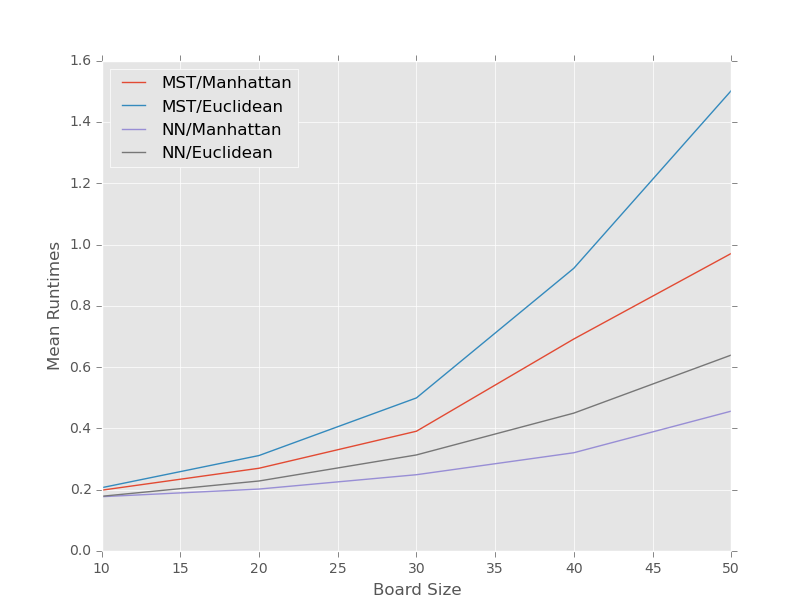
\includegraphics[width=0.45\textwidth]{runtimes.png}
    \caption{Mean of runtimes for variable-width boards with a fixed number of objectives}
    \label{runtimes-fig}
\end{figure}

\begin{figure}[h!]
    \centering
    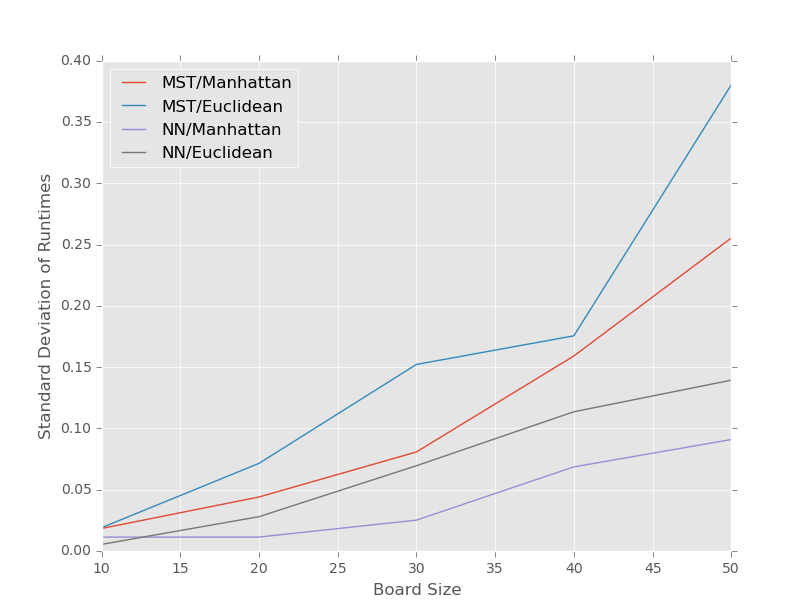
\includegraphics[width=0.45\textwidth]{variability.png}
    \caption{Standard deviation of runtimes for variable-width boards with a fixed number of objectives}
    \label{variability-fig}
\end{figure}

The time complexity of the single-objective A* algorithm is $O(b^d)$ where $d$
is the depth of the optimal path to the nearest goal and $b$ is the average
branching factor.  In practice, we assume $b = 3$ since for any node, there are
three neighbors that can be expanded.  For the multi-objective procedures that
invoke single-objective A*, the nearest-neighbor strategy has time complexity
$O(g)$ and the minimum spanning-path strategy has time compl exity $O(g^2)$
where $g$ is the number of goals and we assume an average constant cost of
calls to single-objective A* by amortizing over the goals.

We observe agreement between the empirical runtime data and the expected
theoretical perf ormance of the algorithms-heuristic combinations.  However, in
future work we would like to explore larger boards and vary the number of obj
ectives to put this claim on firmer footing.


\subsection{Optimality}
The A* algorithm is guaranteed to return the shortest path from a start to end
objective if the heuristic used in admissible.  Both the manhattan and
euclidean heuristic we developed are admissible for this search problem.  By
using the nearest goal, we are guaranteed to find the shortest path to {\em
any} goal.  Additionally, the euclidean distance and manhattan distance will
always be less than the or equal to the actual cost of reaching a goal node.
This is true for Euclidean distance because it calculates the straight line
distance between a start and goal node.  The straight line between any two
points is the shortest path between those points.  The manhattan distance will
also underestimate the cost of reaching a goal because it calculates distance
based on the same rules that the cat ues to move (i.e., can only move
horizontally or vertically.)  The manhattan heuristic also ignores obstacles,
so it will be less than or equal to the actual distance between a start and
goal.

The Nearest Neighbor multi-objective heuristic for this search problem is not
always optimal.  However, it often produces paths which are very close to
optimal.  The reason for non-optimality is that the algorithm will always
choose the path to the nearest goal to the current position.  This does not
account for the distribution of the remaining goals on the map.  As an example,
figure~\ref{nonopt} shows an input map and the non-optimal solution found by
the Nearest Neighbor heuristic.

The Minimum Spanning Path multi-objective heuristic will always find the
optimal path, but at the cost of time complexity.  Because this heuristic
computes the cost of all possible paths through the start point and goals, it
takes much longer to compute with large boards.  However, it will always
produce the most optimal path.  The optimal path determined by this heuristic
for the same map as in figure~\ref{nonopt} can be seen in figure~\ref{opt}.

\begin{figure}[t]
    \centering
    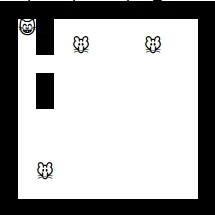
\includegraphics[width=0.4\textwidth]{map_mo.jpg}
    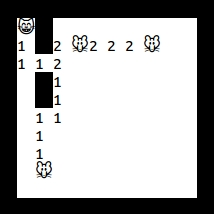
\includegraphics[width=0.4\textwidth]{map_mo_nonopt.jpg}
    \caption{An example multi-objective map and the Nearest Neighbor
heuristic's non-optimal solution.  Path length: 23}
    \label{nonopt}
\end{figure}
\begin{figure}[t]
    \centering
    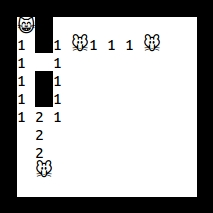
\includegraphics[width=0.4\textwidth]{map_mo_opt.jpg}
    \caption{The optimal solution found from the Minimum Spanning Path
heuristic.  Path length: 22}
    \label{opt}
\end{figure}

\section{Future Work}
The work we have presented in this report is complete for the purposes of
cat-and-mouse problem.  However, as the size and complexity of the problem
becomes larger, our methods will need to be expanded and optimized to allow for
faster computation of a shortest path.  In order to accomodate very large
boards and high dimension boards, the combinatorial method of the MSP heuristic
will become increasingly slow.  Optimizations can be made by reducing the
number of paths which are tested.  For example, rather than testing every
possible path, some of which may not be connected, build and test only paths
which touch every goal.  Additionally, parallelizing the multi-objective
heuristics with MPI or OpenMP would give a substantial increase in performance.

\section{Conclusion}
We have explored the impact of heuristic choice on a multi-objective search
problem utili zing the A* search algorithm.  Multiple heuristics for both
single-objective A* and the multi-objective routine utlizing A* are examined
theoretically and tested for runtime performance.  In addition to our
implementation of A* and the heuristics, our application provides diverse
methods for constructing instances of the search problem and allows future
developers to extend the solvers we provide by adding their own heuristics and
multi-objective strategies.


%\bibliographystyle{IEEEtran}
%\bibliography{bibliography}

\end{document}
